\documentclass[12pt,  english, makeidx, a4paper, titlepage, oneside]{book}
\usepackage{babel}
\usepackage{fancyhdr}
\usepackage{fancyvrb}
\usepackage{makeidx}
\usepackage{titlesec}
\usepackage{listings} 
\usepackage{color}
\usepackage{hyperref}
%\hypersetup{colorlinks=true,linkcolor=red}
\usepackage{mathtools}
\usepackage{psfrag}
\usepackage{booktabs}
\usepackage{tabularx}
\usepackage{array}
\usepackage{colortbl}
\usepackage{subfig}
\usepackage[tight,italian]{minitoc}
\usepackage{epigraph}
\usepackage{lmodern}
\usepackage[T1]{fontenc}
\usepackage{lettrine}
\usepackage{varwidth}

\usepackage{alltt}
\usepackage{xcolor}


\definecolor{dkgreen}{rgb}{0,0.6,0}
\definecolor{gray}{rgb}{0.5,0.5,0.5}
\definecolor{mauve}{rgb}{0.58,0,0.82}

\lstset{
  language=C,
  aboveskip=3mm,
  belowskip=3mm,
  showstringspaces=false,
  columns=flexible,
  basicstyle={\footnotesize\ttfamily},
  numbers=none,
  numberstyle=\tiny\color{gray},
  keywordstyle=\color{blue},
  commentstyle=\color{dkgreen},
  stringstyle=\color{mauve},
  breaklines=true,
  breakatwhitespace=true,
  tabsize=3
}

\newenvironment{scripting}
{\begin{list}{}{\setlength{\leftmargin}{1em}}\item\scriptsize\bfseries}
{\end{list}}

\newenvironment{listato}{\footnotesize}
                        {\normalsize }


%\pagestyle{empty}

%\textwidth 15.5cm
\textheight 23cm
\topmargin -1cm
%\oddsidemargin -0.5cm
\linespread{1.1}

\pagestyle{fancy}
\lhead{}
\chead{Operating Systems}
\lfoot{}
\cfoot{}
\rfoot{}
\rhead{\thepage}

\usepackage{graphicx}
\usepackage{amsmath}
\usepackage{amsfonts}
\usepackage{amsthm}
\usepackage{amssymb}
\usepackage{float}
%\oddsidemargin -1.1cm

\titleformat{\chapter}[display]
{\normalfont\Large\filcenter\sffamily}
{\titlerule[0.5pt]%
\vspace{1pt}
\titlerule
\vspace{1pc}
\LARGE\MakeUppercase{\chaptertitlename} \thechapter
}
{1pc}
{\titlerule
\vspace{1pc}
\Huge}

\graphicspath{{Pictures/}}

\newcommand{\SubSubSection}[1]{\subsubsection{\bf Exercise   ~#1}}

\newcommand{\homework}[1]{\subsubsection{\bf Homework   ~#1}}

\newcommand{\Solution}{\subsubsection{\bf Solution}}

\makeindex
\begin{document}
	\frontmatter
	\begin{titlepage}
		\vspace{2cm}
		\centerline{
		
\includegraphics[width=2cm]{./Pictures/logopoli}}
		\smallskip
		\centerline{\LARGE Politecnico di Torino}
		\bigskip
		\centerline{\Large III Facolt\`a di Ingegneria}
		\vspace{4cm}
		\centerline{\Huge\sf Multi-thread Blowfish algorithm implementation}
		\bigskip
		\centerline{\Large\bfseries\sf Operating Systems}
		\vspace{3cm}
		\centerline{\Large Master degree in Electronic Engineering}
		\vspace{4.4cm}


%%%%%%%%%%%%%%%%%%%%%%%%%%%%%%%%%%%%%%%%%%%%%%%%%%%%%%%
% AUTHORS
% Change the name of the Group participants here
%
\begin{center}
\textbf{	Renzi Alessandro 197783}
\end{center}						
%
%%%%%%%%%%%%%%%%%%%%%%%%%%%%%%%%%%%%%%%%%%%%%%%%%%%%%%
		\vspace{1cm}
		\centerline{\small\today}
	\end{titlepage}

%%%%%%%%%%%%%%%%%%%%%%%%%%%%%%
%content
	\tableofcontents

%%%%%%%%%%%%%%%%%%%%%%%%%%%

	\mainmatter
	\lstset{language=C}

%%%%%%%%%%%%%%%%%%%%%%%%%%%%%%


\chapter{Introduction} \label{introduction}
The aim of this project is to realize a program able to encrypt and decrypt a file using a multi-threaded implementation of the Blowfish algorithm.\\
The user must be able to specify with command line parameters:

\begin{itemize}
 \item If the program should encrypt or decrypt
 \item The input file name
 \item The cryptographic key
 \item The output file name
 \item The number of threads
 \end{itemize}  

The program have to be implemented in C programming language and must also print the total execution time for performance analysis purposes.


\chapter{Blowfish} \label{blowfish}
\section{Algorithm}
The Blowfish algorithm is a symmetric block cipher designed in 1993 by Bruce Schneier as a fast, free alternative to existing encryption algorithms, it operates on 64 bits blocks and takes a variable-length key, from 32 bits to 448 bits (which correspond to 4-56 bytes).
More precisely it is a 16-round Feistel cipher. 

\begin{figure}[H]
\centering
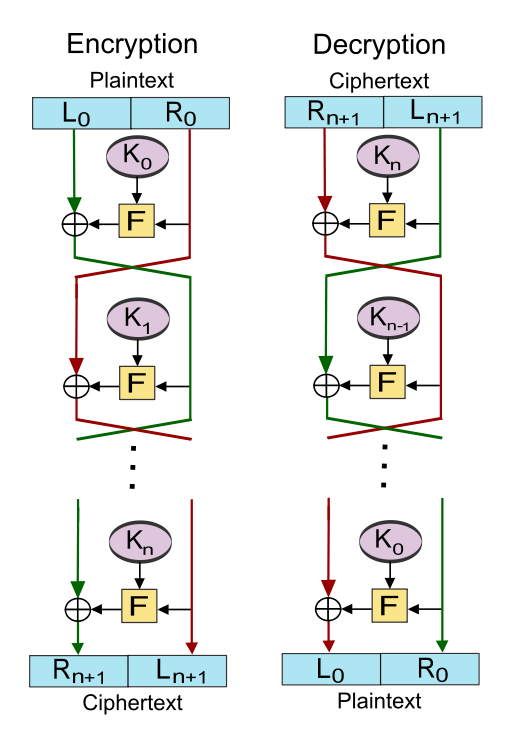
\includegraphics[scale = 0.4]{./Pictures/Feistel_cipher} % x compreso tra 0 e 1
\caption{Feistel cipher}
\label{fig:Feistel cipher}
\end{figure}

Blowfish, unlike DES, uses key-dependend S-boxes, which make it stronger.

\begin{figure}[H]
\centering
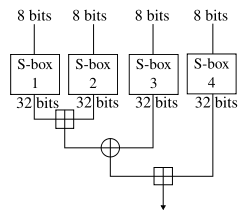
\includegraphics[scale = 0.6]{./Pictures/Blowfish_F_Function} % x compreso tra 0 e 1
\caption{F function}
\label{fig:F function}
\end{figure}

\section{Initial implementation}
Since cryptography is very a complex subject and it's very easy to introduce bugs or vulnerabilities while implementing such an algorithm, I choose to start from the single-threaded reference implementation written by Paul Kocher (https://www.schneier.com/code/bfsh-koc.zip), which has already been verified and tested, and work to make it multi-threaded.
The oroginal API is composed of three functions:

\begin{center}
\begin{lstlisting}
void Blowfish_Init(BLOWFISH_CTX *ctx, unsigned char *key, int keyLen);
void Blowfish_Encrypt(BLOWFISH_CTX *ctx, uint32_t *xl, uint32_t *xr);
void Blowfish_Decrypt(BLOWFISH_CTX *ctx, uint32_t *xl, uint32_t *xr);
\end{lstlisting}
\end{center}

The first has to be executed at the beginning, before encrypting or decrypting, it initializes the Blowfish context (like the S-boxes) using the provided key. This context structure will have to be passed to the encryption/decryption function along with the 64 bits block.\\
The block has to be passed as a pointer to the two halves associated to the two branch of the Feistel cipher, therefore the data passed to the functions is overwritten by the functions themselves. But the fact that the 64 bits block has to be split is an internal implementation detail which the user of the algorithm doesn't care and should be hidden. So I decided to implement two wrappers which take as arguments only the context and the whole 64 bits block, moreover the block is passed by value and the result is returned, in order to give the programmer the freedom to choose if overwrite the input value or not.

\begin{center}
\begin{lstlisting}
uint64_t BlowfishEncryption(BLOWFISH_CTX *ctx, uint64_t x);
uint64_t BlowfishDecryption(BLOWFISH_CTX *ctx, uint64_t x);
\end{lstlisting}
\end{center}

I also switched the entire implementation to the stdint's types which ensure better stability porting the code on different architectures and more predictable results about the underlying representation of the variables.


\chapter{Multi-threading} \label{multi-threading}
In order to distribute the work among several threads I decided to split the input file into blocks, one per thread, so that the work will be split and distributed equally. This allows to reach the maximum speedup because all the threads will have some work to do and none of them will finish a lot earlier than any other and stop without doing nothing.

\begin{figure}[H]
\centering
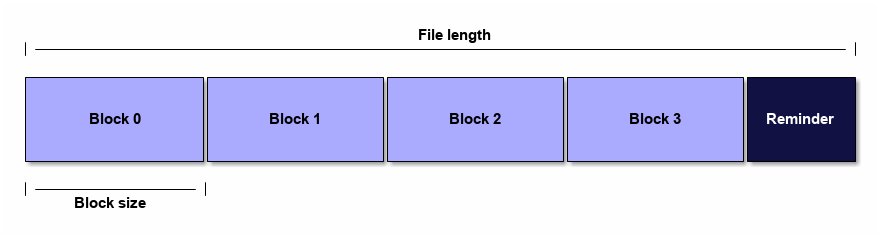
\includegraphics[scale = 0.4]{./Pictures/multithreading} % x compreso tra 0 e 1
\caption{Block subdivision}
\label{fig:multithreading}
\end{figure}

The block size is adjusted in order to be a multiple of 64 bits (the size of the Blowfish's block size), in this way we have a small reminder at the end which we have to handle, I choose to do so in the main thread with a specific portion of code different from the thread's one which may remain neat. Without this adjustment we would had to deal with the reminder of every thread, this would make the code less clean and uselessly complex.\\
In the end the behavior is the following: after the preliminary setup the threads are created, every thread autonomously read the respective portion of the input file 64 bits at a time, encrypt it and write the result in the output file. In the meanwhile the main thread work on the reminder in a similar way, except for a detail, the last 64 bits block.

\section{Padding}
The problem is this: the Blowfish algorithm works only on a fixed size block of 64 bits, but it's unlikely that the input file size is exactly divisible by 8 bytes (64 bits), so once we reach the last block we have to be sure to fill it in some way to make it the right size, the so called \emph{padding} operation.\\
There are several well known ways to handle the padding like to fill with zeros, but most of them make it difficult to distinguish the padding from the actual user data while decrypting. The best protocol I found to deal with this problem is to fill the remaining bytes with the number of bytes to fill, this means embedding the information about the padding size in the padding itself, so we will always be able to correctly decode and trim the output file, an example in figure \ref{fig:padding}.

\begin{figure}[H]
\centering
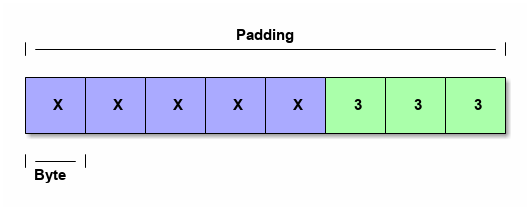
\includegraphics[scale = 0.5]{./Pictures/padding} % x compreso tra 0 e 1
\caption{Padding example (three bytes to be filled)}
\label{fig:padding}
\end{figure}

\subparagraph{Corner case}
One last thing to be noted is the case in which there is no need of padding, since while decoding we read the last byte to know the padding length, the padding cannot be of length zero, because otherwise, we would have no means to know if actually there is a padding or not. So the rule is that there must always be at least one byte of padding.\\
Now we have to find a way to handle the case in which there is no need to pad (length zero), the only way (that come naturally from the implementation) is to add an entire byte of padding, which will be composed of 8s as in figure \ref{fig:padding8}.

\begin{figure}[H]
\centering
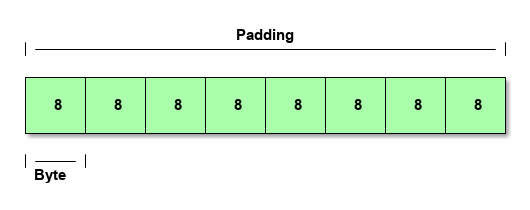
\includegraphics[scale = 0.5]{./Pictures/padding8} % x compreso tra 0 e 1
\caption{Corner case}
\label{fig:padding8}
\end{figure}

\chapter{Buffering} \label{buffering}
After some tests with the earlier version of the software, some performance issues came to light. In particular the execution time was higher with more threads, the exact opposite of the expected behavior. After a deeper analysis of the execution I noted that the CPU was spending more time waiting for I/O from the disk than doing actual work (not very surprising given the well known limits of mechanical hard disks).\\
It becomes immediately clear that reading (and writing) only eight bytes at a time wasn't the best strategy, but on the other hand we could not even load the entire file in RAM (big files may saturate the RAM). So the best way to manage the problem in this case was to load a chunk of data to work on in a temporary buffer, do the encryption, and write out the result. I called these chunks of data \emph{frames}.

\begin{figure}[H]
\centering
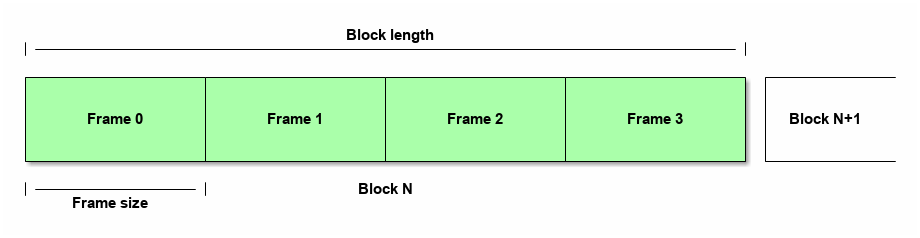
\includegraphics[scale = 0.4]{./Pictures/buffering} % x compreso tra 0 e 1
\caption{Buffering}
\label{fig:buffering}
\end{figure}

So now we have a second level of subdivision within every block, each block is subdivided in frames and only one frame per block (for each thread) is loaded in RAM. Once the work on the current frame is completed the buffer is written out in the output file and the next frame is loaded. This time we don't have any problem of padding, because we simply divide the block size (which is already multiple of eight) by multiples of eight, so everything match and we don't have to worry about the reminder.\\
The frame size is determined dynamically at runtime because if the file to be encrypted is small there is no need to divide the blocks in frames, everything can be kept in RAM. To determine the frame size the algorithm compare the block size with a given threshold, if the block is smaller than the threshold we store the entire block in RAM, otherwise we divide it by eight and compare again, we keep dividing by multiple of eight until we reach a value lower than the threshold.\\
After some tests it turns out that the threshold value, over a certain point, doesn't affect the resulting performance and even a value small as 2MB allows the same performance as any higher value.\\
In the end this proves to be a very valid solution which lead to a big performance gain maintaining a low RAM usage.

\chapter{Implementation} \label{implementation}
\section{Software interface}
The software interface is the following:
\begin{itemize}
\item A character, 'e' or 'd', to select the \textit{\textbf{e}ncryption} mode or the \textit{\textbf{d}ecryption} mode
\item The input file name
\item The key (from 4 to 56 characters without spaces)
\item The output file name
\item The number of threads to use to parallelize the work
\end{itemize}


\section{Preliminary setup}
At the very beginning the CLI arguments are read and stored in the respective variables, then checked for errors, like the number of arguments, the  provided mode flag being either 'e' or 'd' and not another character, the key length, etc...\\
The input file (if exists) is opened, the output one is created and the Blowfish context is created in the \textbf{ctx} variable of type \emph{BLOWFISH\_CTX}.\\

\subsection{Parameter computing}
Subsequently the input file is subdivided in blocks (after reading its length). The block size is determined dividing the file length by the number of threads and then adjusting it to be multiple of eight.\\
After this the reminder size is computed according to this formula:

\begin{scripting}
\begin{verbatim}
reminder size = input file length - (block size * max threads)
\end{verbatim}
\end{scripting}

But we still have to take out the last 64 bits block to be padded, so we compute the effective reminder size (called \emph{aligned}):

\begin{scripting}
\begin{verbatim}
reminder size aligned = reminder size - (reminder size % 8)
\end{verbatim}
\end{scripting}

At this point it's easy to obtain the padding size:

\begin{scripting}
\begin{verbatim}
padding size = 8 - (reminder size % 8)
\end{verbatim}
\end{scripting}

Note that this last formula is sufficient to be consistent with the protocol explained earlier, if the reminder size is already aligned there is no need of padding but the protocol requires an entire byte of padding, this is the behavior that come naturally from the formula.\\
At this point the frames number and size are computed, the algorithm starts with one frame and an initial frame size equal to the block size. If the frame size is smaller than the threshold we finish here. On the contrary, if the size is greater than the threshold we increment the frames number to eight and compute the frame size:

\begin{center}
\begin{lstlisting}
for(frame_number = 8; frame_size < frame_threshold; frame_number+=8)
{
	frame_size = block_size / frame_number;
}
\end{lstlisting}
\end{center}

We keep looping (and dividing) until the frame size is lower than the threshold.


\subsection{Thread creation}
Here the thread pool is created and the read and write mutex (explained later) initialized.\\
Since the thread creation function takes only a pointer to the argument to be passed to the thread function and the only information needed to be passed as argument is the block number on which to work we create an array initialized with numbers from zero to the threads number minus one (0,1,2,3,4,5,6,7,...,max threads-1). Then the reference to each element of the array is passed to the thread, this allows to generalize to any number of threads.\\
After the initialization of the array the threads are created, if there is an error during the thread creation a message is printed on \textbf{stderr} and the program terminates with failure.


\section{Thread implementation}
As first step each thread reads the block number on which works on from the argument, then with this computes the base address of the block:

\begin{scripting}
\begin{verbatim}
base = block size * block number
\end{verbatim}
\end{scripting}

The buffer big as a frame is allocated.\\
The algorithm is composed of two nested loops, the outermost range over every frame of the block, the innermost range over each 64 bits block of the frame encrypt/decrypt it.\\
When we land on a new frame we first read it from the hard disk into the buffer. This is done  by means of the \emph{fseek()} and \emph{fread()} functions. The first set the file cursor on the current frame, the second read it and store it into the buffer. Since these the cursor is only one per file we have to protect these two consecutive operations with a mutex so that the reading operation cannot be interrupted by another thread which changes the cursor position.\\
Even though a process can open a file multiple times, would be counterproductive to read multiple frames simultaneously because mechanical hard disks performs a lot better doing sequential I/O operations (this is the reason that made framing necessary), and switching from a frame to another before finishing the current could nullify the advantages of the buffering.\\
Once the frame buffering is finished we enter the innermost loop which takes each 64 bits block, encrypt/decrypt it according to the mode flag and write back the result into the buffer.\\
When the frame is completely managed we write the buffer into the output file and check for errors in the writing procedure.\\
Then we clean up the memory and terminate the thread.

\section{Reminder and padding}
While the new created threads works on the blocks, the main thread proceed to work on the reminder, the algorithm is basically the same as the thread's one except that, since the reminder is very small, there is no need of buffering. But still there is the need of protecting the readings and writings with the mutex.\\
Once the reminder (except the padding) is handled the main thread waits for the other threads to terminate with the syscall \emph{pthread\_join()}.\\
Then the main (and now only) thread can proceed with the padding, this operation unlike the rest differ significantly in case of encryption or decryption.

\subsection{Encryption padding} 
In case of encryption we first read the last bytes (now there is only one thread, so there is no need of mutex protection), then we clear the bytes to be padded and after that we write the actual padding by means of an OR operation of a suitably shifted value (the padding size as explained earlier).\\
Now that also the last 64 bits block is complete we can encrypt it and then write it into the output file.

\subsection{Decryption padding} 
In case of decryption at this point we have already decrypted the last 64 bits block containing the padding and wrote it into the output file. So it is sufficient to move the file cursor one byte back and read the padding length (the protocol explained earlier guarantee that the last byte is always the padding length), once we know the padding length it is easy to trim the file to the right length using the \emph{truncate()} syscall.



\section{Benchmark}
The benchmark is based on the \emph{clock\_gettime()} syscall, it stores the current time (with very high resolution) into a variable of type \emph{struct timespec} which is defined in this way:

\begin{center}
\begin{lstlisting}
struct timespec 
{
        time_t   tv_sec;        /* seconds */
        long     tv_nsec;       /* nanoseconds */
};
\end{lstlisting}
\end{center}

Using two variables: \textbf{start} and \textbf{end}, the first set at the beginning and the second at the end, and a function to compute the difference, it is possible to measure the execution time of the program.

\begin{center}
\begin{lstlisting}
int64_t timespecDiff(struct timespec *timeA_p, struct timespec *timeB_p)
{
  return ((timeA_p->tv_sec * 1000000000) + timeA_p->tv_nsec) -
           ((timeB_p->tv_sec * 1000000000) + timeB_p->tv_nsec);
}
\end{lstlisting}
\end{center}

The benchmark sections are enclosed into \emph{\#ifdef BENCHMARK} blocks in order to make easy to enable or disable it by simply defining or not the symbol \emph{BENCHMARK}.

\section{Memory cleaning}
Before exiting and before terminating the threads all the memory is freed but only after writing zeros in all the variables and data structures used, like the threads buffer, the blowfish's context, etc. This avoids to leave traces in RAM after the execution that may allow an attacker to find the key.

\chapter{Benchmark} \label{benchmark}
The tests have been conducted on a linux machine, kernel SMP 3.13.11, equipped with a Quad core CPU Intel Core i7-4700MQ CPU @ 2.40GHz (Turbo-Boost up to 3.4GHz) with support for HyperThreading technology which enables each core to handle efficiently up to two threads.\\
The test consists of encrypting a file, decrypting it, and comparing the decrypted one with the original to check functional correctness. The files used for the tests range in dimension from few hundreds of KB to 4GB, but there is no limit on the size of the input file apart from the kernel limit and the upper bound imposed by the 64 bits variable for addresses.\\
Every file have been tested with 1, 2, 4 and 8 threads (the maximum parallelism allowed by the hardware).\\
The results are the following:

\begin{figure}[H]
\centering
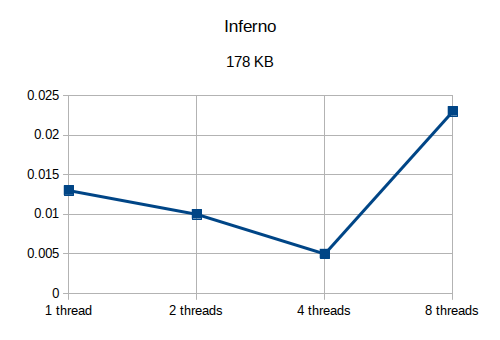
\includegraphics[scale = 0.8]{./Pictures/Inferno} % x compreso tra 0 e 1
\caption{Inferno}
\label{fig:Inferno}
\end{figure}

\begin{figure}[H]
\centering
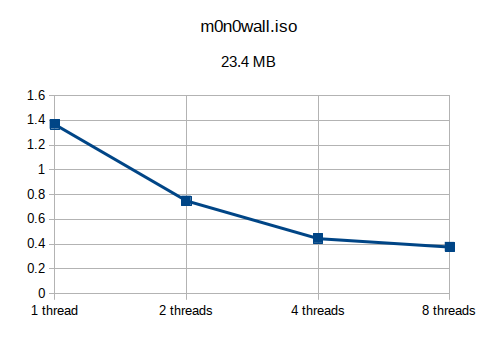
\includegraphics[scale = 0.8]{./Pictures/m0n0wall} % x compreso tra 0 e 1
\caption{m0n0wall}
\label{fig:m0n0wall}
\end{figure}

\begin{figure}[H]
\centering
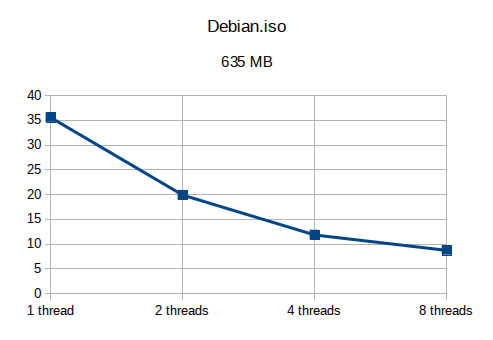
\includegraphics[scale = 0.8]{./Pictures/Debian} % x compreso tra 0 e 1
\caption{Debian}
\label{fig:Debian}
\end{figure}

\begin{figure}[H]
\centering
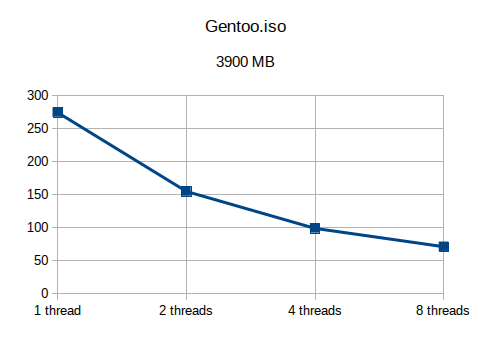
\includegraphics[scale = 0.8]{./Pictures/Gentoo} % x compreso tra 0 e 1
\caption{Gentoo}
\label{fig:Gentoo}
\end{figure}

As we can see, apart for an anomaly in the first test due to the fact that the file was really too small for such an high number of threads, the algorithm scales very well and can handle well also very big files.\\
Doubling the number of threads lead to a speedup which range from 1.4 to 1.82.

\subparagraph{Script}
The test script is the following:

\begin{scripting}
\begin{verbatim}
#!/bin/sh
#set -xv

# WARNING: diff fail in case of final new line in input file

BUILD_DIR=./build
TEST_DIR=./test

TEST_FILE=test_input
KEY="0000000000000000"
MAX_THREADS=8
DEBUG=0

EXECUTABLE=$BUILD_DIR/blowfish-multithread
INPUT=$TEST_DIR/$TEST_FILE
ENC_OUTPUT=$TEST_DIR/enc_output
DEC_OUTPUT=$TEST_DIR/dec_output

ENC_LOGFILE=$TEST_DIR/enc.log
DEC_LOGFILE=$TEST_DIR/dec.log



if [ "$DEBUG" == "1" ]; then
	EXECUTABLE="gdb --args $EXECUTABLE"
fi


echo "clean"
if [ -a "$ENC_OUTPUT" ]; then
	rm "$ENC_OUTPUT"
fi

if [ -a "$DEC_OUTPUT" ]; then
	rm "$DEC_OUTPUT"
fi

echo "encrypt"
$EXECUTABLE "e" "$INPUT" "$KEY" "$ENC_OUTPUT" "$MAX_THREADS" #> "$ENC_LOGFILE"
echo ""

echo "decrypt"
$EXECUTABLE "d" "$ENC_OUTPUT" "$KEY" "$DEC_OUTPUT" "$MAX_THREADS" #> "$DEC_LOGFILE"
echo ""

echo "comparing"
if diff -B -b -E -Z "$INPUT" "$DEC_OUTPUT" >/dev/null ; then
	echo -e "\e[00;32mOK\e[00m"
else
	echo -e "\e[00;31mDifferent\e[00m"
fi
\end{verbatim}
\end{scripting}


\end{document}